\documentclass{beamer}

\usepackage{amssymb,amsmath,amsfonts,amsthm}
\usepackage{mathrsfs}

\title{Learning Lean Seminar}
\author{Matej Penciak}
\institute{Northeastern University}
\date{February 4, 2022 \\ Slides available at: \\ https://github.com/mpenciak/Lean-Seminar-Sp2022}

\begin{document}

% Title Slide
\frame{\titlepage}

\begin{frame}
    \frametitle{What is Lean?}
    \pause
    ``Lean is a functional programming language that makes it easy to write correct and maintainable code. {\bf You can also use Lean as an interactive theorem prover}. Lean programming primarily involves defining types and functions.''
    (https://leanprover.github.io/about/)
\end{frame}


\begin{frame}
    \frametitle{What is an interactive theorem prover/proof assistant?}
    \pause
    It's a tool to that helps bridge the gap between proofs that can be understood by humans, and proofs that can be understood by computers.

    \vspace{20pt}
    \pause
    This answer is purposefully vague, and before we can make it more precise we need to first understand what constitutes a mathematical proof.
\end{frame}

\begin{frame}
    \frametitle{What is a proof?}
    \pause
    The answer to this is tricky, and the definition has changed over the course of the history of mathematics!
\end{frame}

\begin{frame}
    \frametitle{Proofs in ancient Greece}
    \begin{center}
        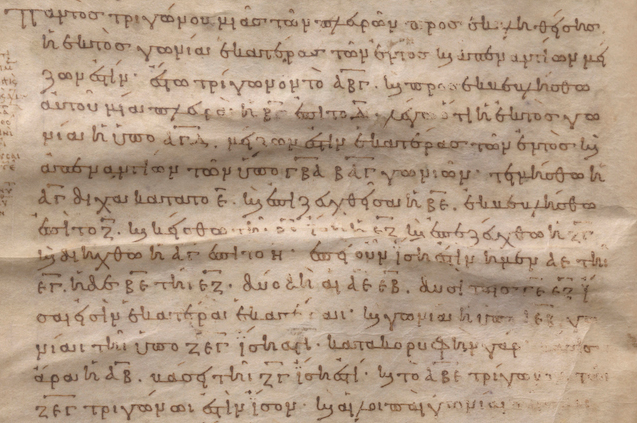
\includegraphics[scale=.3]{img/elements.png}
    \end{center}

    \pause
    Prop. 16: Upon one of the sides of any triangle being extended, the external angle is larger than each of the interior and opposite angles.
    
    Let there be a triangle, ABG, and let one side of it, BG, be extended to D. I say that the exterior angle, that by AGD, is larger than each of the interior and opposite angles, the angles by GBA, BAG. Let AG be bisected at E, and let BE, being joined, be extended on a straight-line to Z, and let \ldots
\end{frame}

\begin{frame}
    \frametitle{Proofs in the age of enlightenment}
    \begin{center}
        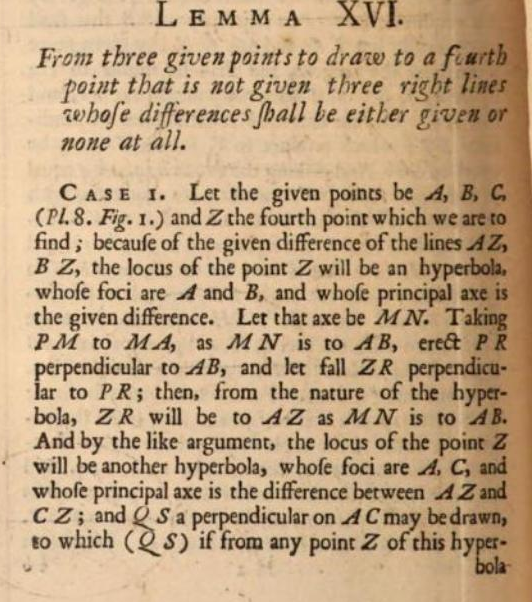
\includegraphics[scale=.4]{img/mathematica.png}
    \end{center}
\end{frame}

\begin{frame}
    \frametitle{Proofs in the early 20th century}
    \begin{center}
        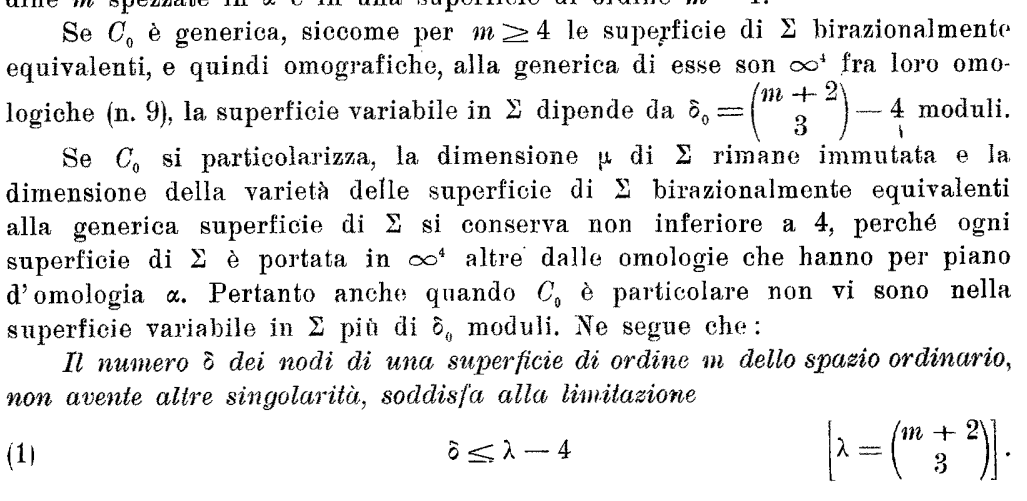
\includegraphics[scale=.35]{img/severi.png}
    \end{center}
\end{frame}

\begin{frame}
    \frametitle{Proofs now}
    \begin{center}
        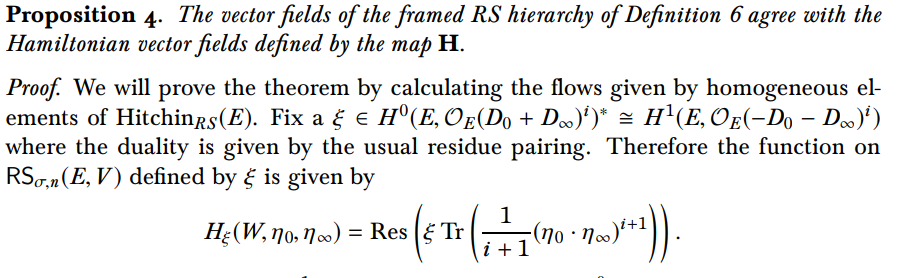
\includegraphics[scale=.4]{img/mypaper.png}<-1>
        \pause
        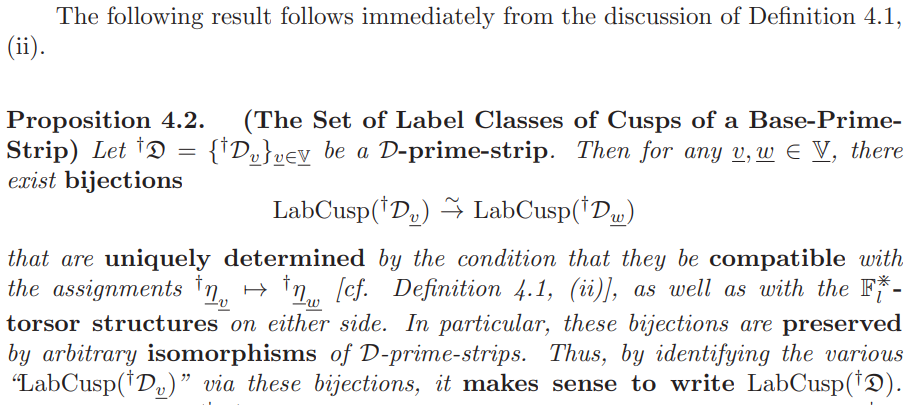
\includegraphics[scale=.4]{img/IUT.png}<2->
    \end{center}
\end{frame}

\begin{frame}
    \frametitle{Proofs in the future?}
    \begin{center}
        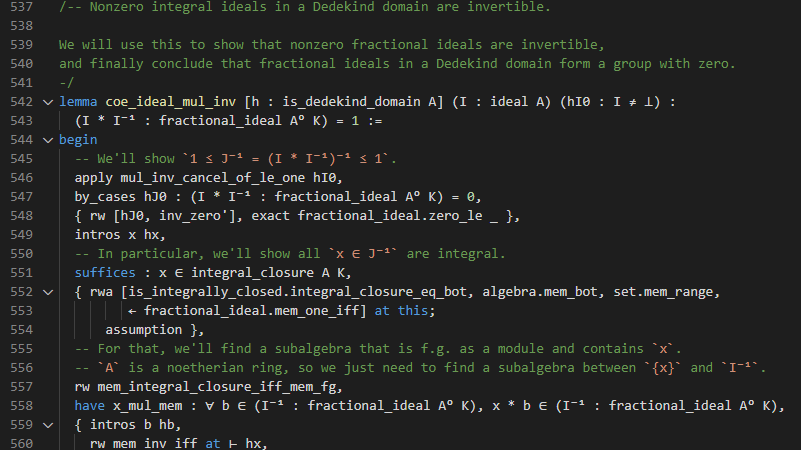
\includegraphics[scale=.5]{img/lean.png}
    \end{center}
\end{frame}

\begin{frame}
    \frametitle{What is proof formalization?}
    In a very simplified form, Lean has a small kernel of the essential rules of logical deduction.

    \pause
    \vspace{20pt}
    The goal of proof formalization is to implement the proofs of all of the major mathematical results starting from these basic principles.

    \pause
    \vspace{20pt}
    The ongoing proof formalization project in Lean is named mathlib (https://github.com/leanprover-community/mathlib)

    \pause
    \vspace{20pt}
    This should not be confused with proof by checking all the cases! (Like the proof of the 4 color theorem)
\end{frame}

\begin{frame}
    \frametitle{Why formalize proofs?}
    \begin{enumerate}
        \item<1-> Catch any errors we made along the way (not as many as you'd think)
        \item<2-> Develop insights into how results are proven. A once in human history chance to re-factor all of mathematics!
        \item<3-> Help future mathematicians to prove new theorems by developing tools along the way.
    \end{enumerate}
\end{frame}

\begin{frame}
    \frametitle{Formalize all the math!}
    \begin{center}
    
\includegraphics[scale=.35]{img/formalize.png}
    \end{center}
    {\bf Q}: Does that mean we have to implement every theorem into Lean by hand?
    \pause

    {\bf A}: (short answer) Yes!

    \pause
    {\bf A}: (long answer) Probably! At least for now.
\end{frame}

\begin{frame}
    \frametitle{Other interactive theorem provers}
    \begin{enumerate}
        \item Agda
        \item Coq
        \item HOL
        \item Idris
        \item ... Many more!
    \end{enumerate}
    \vspace{20pt}
    \pause
    Why Lean then? 
    
    \vspace{20pt}
    \pause
    Lean just feels right for what I (a mathematician) wants to do (prove theorems). \pause A specific example is quotients! \pause And sheaves \pause and schemes \pause and triangulated categories \pause and...

    \vspace{20pt}
    \pause
    The biggest part is the community! So many resources to learn from, and everyone is so friendly and so excited, it's hard not to get swept up in the hype!
\end{frame}

\begin{frame}
    \frametitle{Where do I fit into all this?}
    There's a lot of math, so everyone little bit helps!

    \vspace{20pt}
    \pause
    There's a lot of parts of the undergraduate curriculum that have yet to be formalized.

    \vspace{20pt}
    \pause
    Might as well start now. 
\end{frame}

\begin{frame}
    \frametitle{Plan for the semester}
    \begin{enumerate}
        \item Learn about the Lean platform by attending short talks like this, and working in groups on small projects
        \item Learn about specific parts of the mathlib (kind of like learning a new API or module)
        \item Pick a theorem, and try to try to formalize and work in groups to add it to mathlib!
        \pause
        \item<2-> (for mathematicians) Learn all of the useful tools that computer scientists have been hiding from us (version control with git, SAT solvers)
        \item<2-> (for computer scientists) Maybe learn some math along the way? 
    \end{enumerate}
\end{frame}

\begin{frame}
    Enough slides, lets prove some theorems!
\end{frame}
        
\end{document}